\documentclass[12pt]{article}
\usepackage{amsmath}
\usepackage[english]{babel}
\usepackage{graphicx}
\usepackage{subfig}

\title{Detecting House Numbers in Street View Imagery using Convolutional Neural Networks}
\author{Matthew Peyrard}
\date{\today}

\begin{document}
\maketitle

\section{Definition}
\subsection{Project Overview}
This project is my submission for the Capstone Project section for Udacity's Machine Learning Nanodegree program.
The goal of the project is to automate the task of identifying house numbers from imagery taken from Google's street view cameras.


\subsection{Problem Statement}
The process of \textit{manually} identifying and cataloging such imagery is very expensive due to the scale at which such a process must be applied.
However, if computational resources could be applied to the task with reasonably high accuracy, then the process could be sped up enormously, in addition to the costs saved from not having to hire thousands of people to perform the task manually.
The solution was based on the original paper published by Goodfellow et al. \cite{svhn_original_paper}, utilizing deep convolutional neural networks. 
The standard street view house number dataset \cite{svhn_dataset} was used as a training source for this project.

\subsection{Metrics}
Performance for this task is measured using an accuracy calculation based on a train/test split. 
Every 100 iterations of the training algorithm, the test set is fed into the algorithm and we measure the accuracy. 
No partial credit is provided for the algorithm. 
A prediction is correct if and only if the entire digit is predicted correctly. 
Furthermore, since we are using the method described in the original paper \cite{svhn_original_paper}, the predicted length of the digit must also be correct. 

\section{Analysis}
\subsection{Data Exploration}
The standard Street View House Number dataset\cite{svhn_dataset} was used for training and validation for this project. 
This data set comes with three sets of images: training, testing and extra. 
The training and testing data sets each consists of 33,402 and 13,068 images respectively. 
The extra dataset consists of over 200,000 images that are considered slightly easier, and are used as additional training and validation data. 
Each of these datasets also contains a \textit{Matlab} file that provides the labels and bounding boxes for each of the digits in each image.
For the purpose of this project, the Matlab file was converted into a CSV file that contained the image filename and the digits it contains. 
The bounding boxes were discarded because predicting the positions of the digits was out of scope for this initial version of the project. 
Furthermore, the matlab file was also scrapped (a script was written to convert it to CSV) because loading it took an excessive amount of time.

\begin{figure}[!htb]
\minipage{0.32\textwidth}
	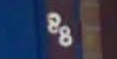
\includegraphics[width=\linewidth]{1046.png}
\endminipage\hfill
\minipage{0.32\textwidth}
	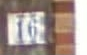
\includegraphics[width=\linewidth]{10.png}
\endminipage\hfill
\minipage{0.32\textwidth}
	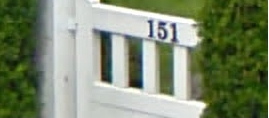
\includegraphics[width=\linewidth]{20.png}
\endminipage\hfill
\caption{Examples of SVHN imagery.}
\label{fig:example_imagery}
\end{figure}

Figure \ref{fig:example_imagery} demonstrates some examples of the kinds of imagery we are dealing with in the SVHN dataset. 
As you can see, there is a lot of variability in both the image size and image quality. 
For example in the center image, we can just barely tell that the first digit is a 1, but it could easily be misconstrued as a 7. 
However, one advantage that is provided by this data set is that digits, while not necessarily front and center, are at least prominent within the image.

Another potential complication is demonstrated by the left-most image, which shows that not all of the individual digits are lined up nicely.
Some of them are stacked diagonally or even vertically, and the neural network must be able to figure this out. 

\subsection{Exploratory Visualization}
The first interesting property about the SVHN data set is the distribution of digit lengths across the different partitions (training, testing and extra).
Each image has one to five digits in the house number.
However, as shown in Figures \ref{fig:digit_length_plots} and \ref{fig:digit_length_table}, the digit lengths are not all equally represented by the training data.
This is likely representative of the relative probability of seeing a house number of each given length, but also raises the potential for the model to learn a bias towards common digit lengths, or against those less common ones.
As the data shows, digit lengths of two and three are far more common, while five digit house numbers are almost non-existent.

\begin{figure}[!htb]
\centering
\subfloat[Training\label{fig:train_digit_length_plot}]{
	\centering
	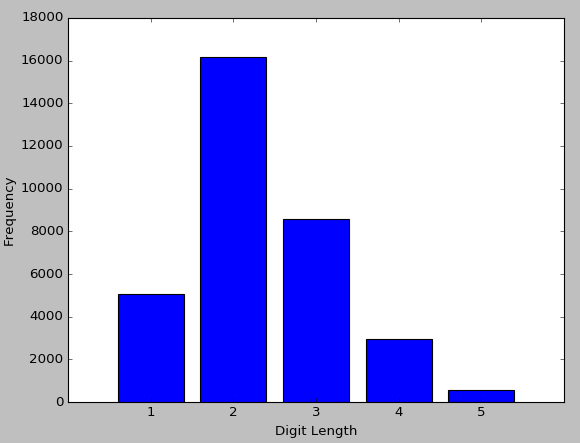
\includegraphics[width=0.45\columnwidth]{train_digit_lengths.png}
}\hfill
\subfloat[Testing\label{fig:test_digit_length_plot}]{
	\centering
	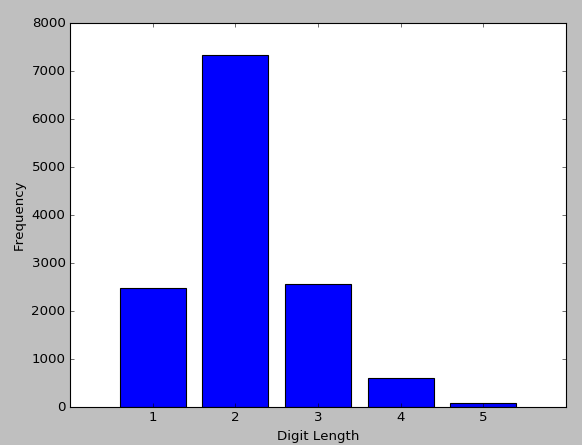
\includegraphics[width=0.45\columnwidth]{test_digit_lengths.png}
}\hfill
\subfloat[Extra\label{fig:extra_digit_length_plot}]{
	\centering
	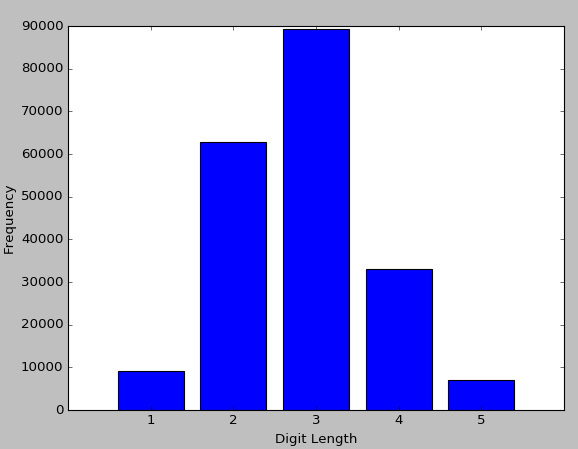
\includegraphics[width=0.45\columnwidth]{extra_digit_lengths.png}
}\hfill
\caption{Distributions of digit lengths for each of the training sets.}
\label{fig:digit_length_plots}
\end{figure}

\begin{figure}[!htb]
\begin{center}
\begin{tabular}{ |c|c|c|c|c|c| }
\hline
       & 1       & 2       & 3       & 4       & 5       \\
\hline
Train  & 15.25\% & 48.48\% & 25.69\% & 8.86\%  & 1.72\%  \\
\hline
Test   & 18.94\% & 56.13\% & 19.56\% & 4.67\%  & 0.70\%  \\
\hline
Extra  & 4.52\%  & 31.19\% & 44.36\% & 16.43\% & 3.48\%  \\
\hline
\end{tabular}
\end{center}
\caption{Ratio of each digit length's presence in its respective data set.}
\label{fig:digit_length_table}
\end{figure}

\begin{figure}[!htb]
\centering
\subfloat[Training\label{fig:train_digit_freq_plot}]{
	\centering
	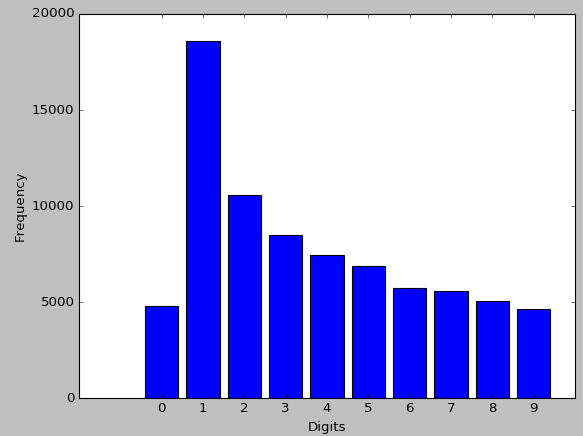
\includegraphics[width=0.45\columnwidth]{train_digit_freq.png}
}\hfill
\subfloat[Testing\label{fig:test_digit_freq_plot}]{
	\centering
	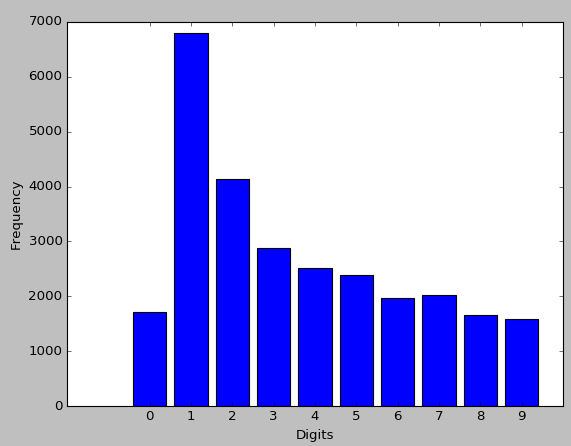
\includegraphics[width=0.45\columnwidth]{test_digit_freq.png}
}\hfill
\subfloat[Extra\label{fig:extra_digit_freq_plot}]{
	\centering
	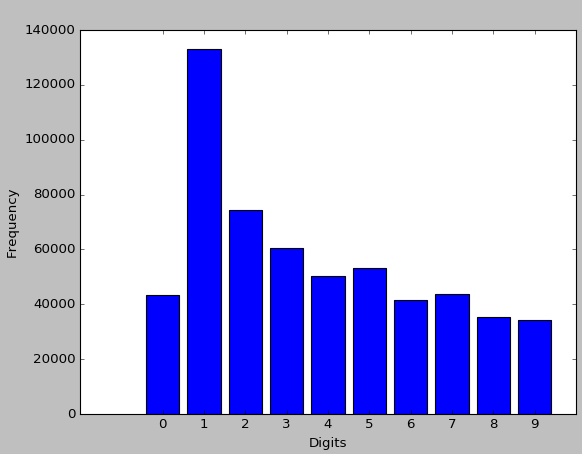
\includegraphics[width=0.45\columnwidth]{extra_digit_freq.png}
}\hfill
\caption{Distributions of individual digit frequencies for each of the training sets.}
\label{fig:digit_freq_plots}
\end{figure}

There is a similar asymmetry with the distribution of the individual digits.
As demonstrated by Figure \ref{fig:digit_freq_plots}, the digit 1 is by far the most common digit across all data sets.
Similar to the digit length bias, this asymmetry creates a potential bias towards the digit 1 in the model's predictions.
Even if there is not a bias, the model may be far more successful in recognizing 1's relative to other digits.

\subsection{Algorithms and Techniques}
In order to solve this problem, a convolutional neural network has been employed.


\subsection{Benchmark}
The performance benchmark that was used to optimize the learning algorithm was the Adagrad optimization algorithm. 
Adam and Adadelta optimizers were also tested, but Adagrad proved to have the highest accuracy on this task.

Since this is a discrete classification problem with a small number of classes, the cross entropy of the predictions and labels was used as a loss function to be minimized.
The cross entropy $H$ of two probability distributions $p$ and $q$ is given by:

\begin{equation}
	H(p,q) = -\sum_{x \in X} p(x) \log q(x)
\end{equation}

where $X = \{0, 1, ..., 9 \}$, representing the ten distinct digit classes we are identifying.
Since the cross-entropy relies on $p$ and $q$ to be probability distributions, we must ensure that our predictions and labels also take the form of probability distributions.

This is simple in the case of the training label, as we can simply use a 1-hot encoded vector, meaning that it is a 10-dimensional vector filled with zeros, except for the entry representing the correct label, which holds a 1.
For example, the following vector would represent a label of 5:

\begin{align}
	\hat{y} &= \begin{bmatrix}
		0 \\
		0 \\
		0 \\
		0 \\
		0 \\
		1 \\
		0 \\
		0 \\
		0 \\
		0 \\
	\end{bmatrix} 
\end{align}

For the model predictions, the final matrix multiply will also provide a 10-dimensional vector.
However, those predictions will be a weighted representation of the relative confidence the model has in each possible prediction.
The problem is that the values of such a vector will not necessarily sum to 1, meaning it is not a valid probability distribution.
We use a standard normalization technique called \textit{softmax} to ensure the values sum to 1, while preserving the relative weighting.
Softmax is defined element-wise as:

\begin{equation}
	S(y)_j = \frac{\exp(y_j)}{\sum_{i=1}^K \exp(y_i)}
\end{equation}

where in this case $K=10$.
This means that our loss function for the $i$-th digit is defined as:

\begin{equation}
	L_i = H(S(y_i), \hat{y}_i)
\end{equation}

where $y_i$ is the model's prediction vector for the $i$-th digit, and $\hat{y}_i$ is the training label 1-hot vector for the $i$-th digit.
Finally, we need to unify these losses into a single function that can be used by the optimizer.
Summing the losses together suffices for this purpose, giving us the final loss function:

\begin{equation}
	\mathcal{L} = \sum_{i=1}^5 L_i
\end{equation}

\section{Methodology}
\subsection{Data Preprocessing}
Two data pre-processing steps were performed for this project. 

The first step is to simply resize each image to $32 \times 32$. This is because neural networks have rigid input shape requirements. The second pre-processing step is a centering operation performed by subtracting the mean of all the pixels in the training data. 

No measures were taken to adjust to compensate for the over-abundance of 2-digit numbers, or for the execess in numbers containing the digit 1. The assumption is that the network should be large enough to learn the difference between the different digits, regardless of their distribution. It is likely that the network will be better at recognizing 1s than for other digits, but this fact shouldn't hinder its ability to recognize other digits.

\subsection{Implementation}
The architecture of the neural network is roughly based on the design outlined in the original paper \cite{svhn_original_paper}.
The network uses eight convolutional layers, with depths of 48, 64, 128 and 160 for the first four layers, and 192 for the final four layers.
This is followed by two fully connected layers with 4096 units each.
The network then splits into five output layers, each one predicting one of the up-to-five digits in the image. 
Each output layer is assigned a static index $i$, and that layer is responsible for predicting the $i$-th digit. 
If the number has fewer digits than $i$, then the output layer will output the null class, which in this case is just the digit 10.
Each output layer is a fully connected softmax classifier.

Every convolutional layer and pre-output fully connected layer uses ReLU\cite{relu} activations followed by dropout\cite{svhn_dropout} and local response normalization\cite{svhn_lrn} layers.
The convolutional kernel size for all convolutional layers was $5 \times 5$, along with a stride of 1.

Max pooling was used twice, once following convolutional layer 4, and again following convolutional layer 8.
Both max pooling layers used $2 \times 2$ windows with a stride of 1.

The Adagrad optimizer was used with an initial learning rate $\alpha_0 = 0.025$, decaying over the course of 50,000 epochs to a final learning rate of 0.0075. 

\subsection{Refinement}
The biggest sources of improvement during this project was the adjustment of the learning rate and increasing the size of the network.
The network was initially half the size of the final architecture, with four convolutional layers, and one fully connected layer.
The learning rate was initially set statically to 0.05, which was good enough to get the model off the ground, but it often got stuck at around 40\% accuracy. 
Such a learning rate was clearly too high to allow the optimizer to find the smaller crevices that lead to higher accuracies. 
In response to this, some major performance improvements were gained by lowering the learning rate to 0.025 and introducing the exponential decay.
This allowed the accuracy to increase to 80\%, however once it reached this point, the network would suddenly jump out of its current optimum, and land somewhere completely sub-optimal. 
This can be seen in Figure \ref{fig:small_network_results}.
Whether this was a Tensorflow bug, or as a result of a flawed architecture, was not discernable.
However, by increasing the network size, in addition to the changes in the learning rate, the accuracy (on the validation set) was able to exceed 90\%. 

There were two methods for this, the most successful one which has been outlined in the Implementation section achieved a peak accuracy of 91\%, which is shown in Figure \ref{fig:best_results}.
The second method was the one outlined in the original paper \cite{svhn_original_paper}, which uses length prediction in place of placeholder digits (for missing digits).
The best results achieved for this method were 90.1\% accuracy, which is outlined in Figure \ref{fig:length_best_results}.

\begin{figure}[!htb]
\centering
\subfloat[Loss\label{fig:best_loss}]{
	\centering
	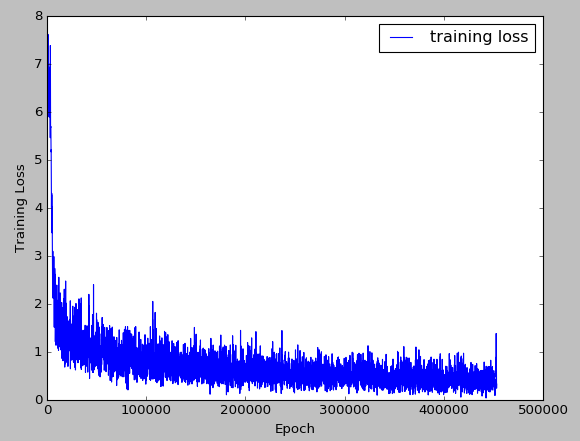
\includegraphics[width=0.45\columnwidth]{length_best_loss.png}
}\hfill
\subfloat[Accuracy\label{fig:best_accuracy}]{
	\centering
	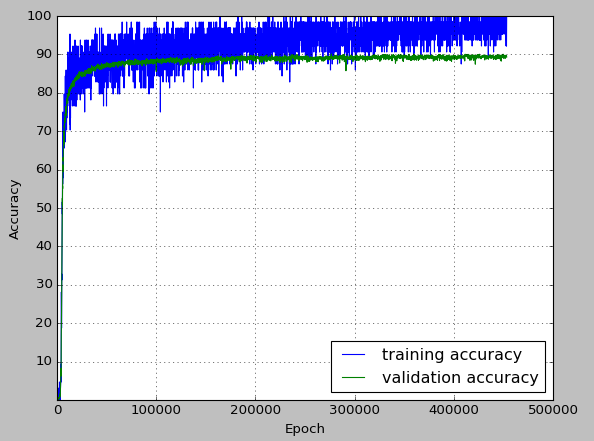
\includegraphics[width=0.45\columnwidth]{length_best_accuracy.png}
}\hfill
\caption{Plot of best run using placeholder digit, $\alpha_0 = 0.025$, 50,000 epoch decay to 0.0075.}
\label{fig:best_results}
\end{figure}

\begin{figure}[!htb]
\centering
\subfloat[Loss\label{fig:lenth_best_loss}]{
	\centering
	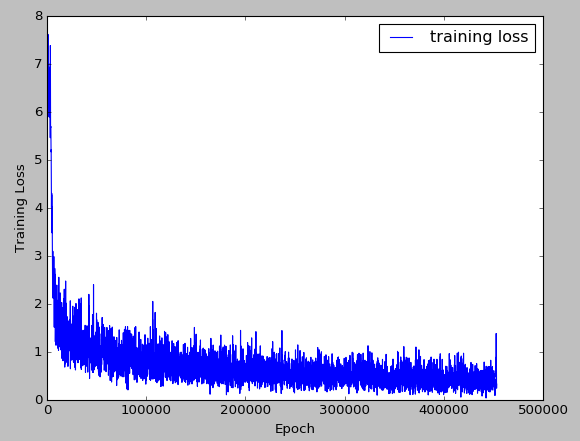
\includegraphics[width=0.45\columnwidth]{length_best_loss.png}
}\hfill
\subfloat[Accuracy\label{fig:length_best_accuracy}]{
	\centering
	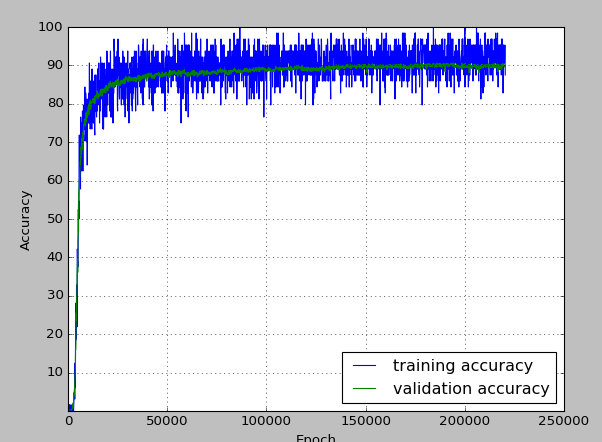
\includegraphics[width=0.45\columnwidth]{best_accuracy.png}
}\hfill
\caption{Plot of best run using length prediction, $\alpha_0 = 0.025$, 50,000 epoch decay to 0.0075.}
\label{fig:length_best_results}
\end{figure}

\begin{figure}[!htb]
\centering
\subfloat[Loss\label{fig:small_best_loss}]{
	\centering
	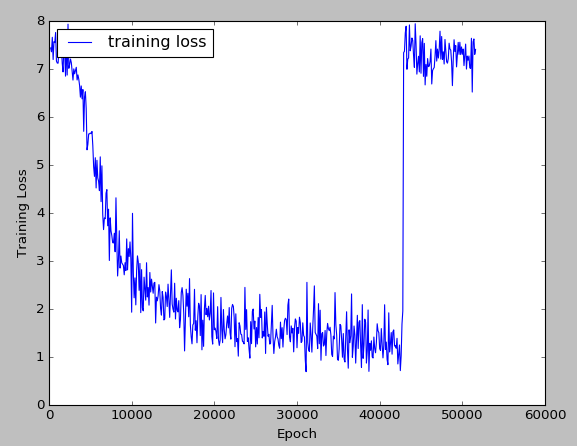
\includegraphics[width=0.45\columnwidth]{small_network_loss.png}
}\hfill
\subfloat[Accuracy\label{fig:small_best_accuracy}]{
	\centering
	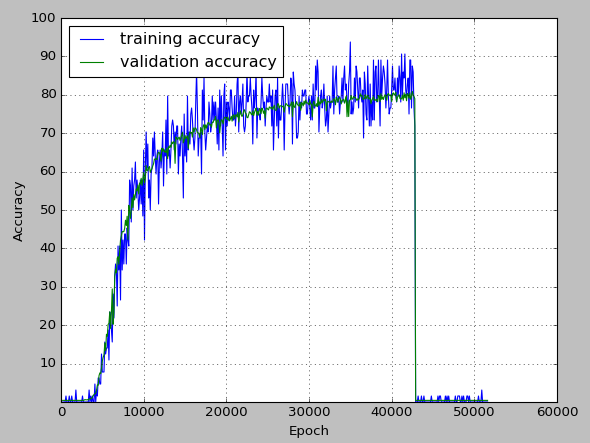
\includegraphics[width=0.45\columnwidth]{small_network_accuracy.png}
}\hfill
\caption{Plot of run using smaller convolutional network, $\alpha_0 = 0.025$, 30,000 epoch decay to 0.001.}
\label{fig:small_network_results}
\end{figure}


\section{Results}
Work in progress.

\subsection{Model Evaluation and Validation}
Work in progress.

\subsection{Justification}
Work in progress.

\section{Conclusion}
Work in progress.

\subsection{Free-Form Visualization}
Work in progress.

\subsection{Reflection}
Work in progress.

\subsection{Improvement}
Work in progress.


\begin{thebibliography}{9}
\bibitem{svhn_dataset} 
Yuval Netzer, Tao Wang, Adam Coates, Alessandro Bissacco, Bo Wu, Andrew Y. Ng 
\textit{Reading Digits in Natural Images with Unsupervised Feature Learning NIPS Workshop on Deep Learning and Unsupervised Feature Learning 2011.}
http://ufldl.stanford.edu/housenumbers/
\bibitem{svhn_original_paper}
Goodfellow, Ian J.; Bulatov, Yaroslav; Ibarz, Julian; Arnoud, Sacha; Shet, Vinay
\textit{Multi-digit Number Recognition from Street View Imagery using Deep Convolutional Neural Networks}
\bibitem{svhn_lrn}
Alex Krizhevsky and Sutskever, Ilya and Geoffrey E. Hinton
\textit{ImageNet Classification with Deep Convolutional Neural Networks}
\bibitem{svhn_dropout}
Nitish Srivastava, Geoffrey Hinton, Alex Krizhevsky, Ilya Sutskever, Ruslan Salakhutdinov
\textit{Dropout: A Simple Way to Prevent Neural Networks from Overfitting}
\bibitem{relu}
R Hahnloser, R. Sarpeshkar, M A Mahowald, R. J. Douglas, H.S. Seung (2000). 
\textit{Digital selection and analogue amplification coesist in a cortex-inspired silicon circuit.}

\end{thebibliography}
	
\end{document}

